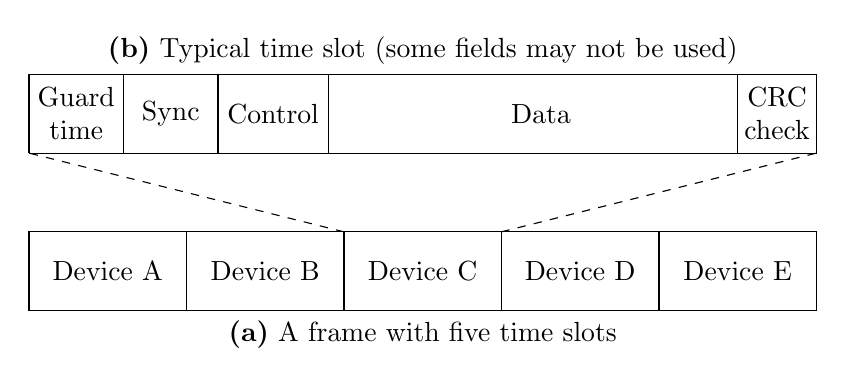
\begin{tikzpicture}[auto]
    \path[draw] (-5,0) -- (-5,1) -- (5,1) -- (5,0) -- (-5,0)
                (-3,1) -- (-3,0)
                (-1,1) -- (-1,0)
                (1,1) -- (1,0)
                (3,1) -- (3,0);
                
    \node at (-4,0.5) {Device A};
    \node at (-2,0.5) {Device B};
    \node at (0,0.5) {Device C};
    \node at (2,0.5) {Device D};
    \node at (4,0.5) {Device E};
    
    \path[draw, dashed] (-1,1) -- (-5,2)
                        (1,1) -- (5,2);
    
    \path[draw] (-5,2) -- (-5,3) -- (5,3) -- (5,2) -- (-5,2)
                (-3.8,2) -- (-3.8,3)
                (-2.6,2) -- (-2.6,3)
                (-1.2,2) -- (-1.2,3)
                (4,2) -- (4,3);
    
    \node[text width=1cm, align=center] at (-4.4,2.5) {Guard\\time};
    \node at (-3.2,2.5) {Sync};
    \node at (-1.9,2.5) {Control};
    \node at (1.5,2.5) {Data};
    \node[text width=1cm, align=center] at (4.5,2.5) {CRC\\check};
    
    \path (-5,3) -- node{\textbf{(b)} Typical time slot (some fields may not be used)} (5,3);
    
    \path (5,0) -- node{\textbf{(a)} A frame with five time slots} (-5,0);
\end{tikzpicture}